\chapter{NUMA Topology Views}
Kapitola se bude zabývat posledním z hlavních vylepšení této práce, tj. přidáním informací o NUMA topologii CPU na systému do KernelSharku. Tato modifikace pak bude hlavně sloužit k vylepšení analýzy trasovacích dat, jelikož budeme jednodušeji schopni určit namáhanou část topologie. Kapitola postupně představí cíle, analýzu řešení, návrh, uživatelskou dokumentaci, návrhy pro rozšíření, kritiku řešení a konečné zhodnocení splnění cílů této modifikace.

%%%%%%%%%%%%%%%%%%%%%%%%%%%%%%%%%%%%%%%%%%%%%%%%%%%%%%%%%%%%%%%%%%%%%%%
\section{Cíle}

\begin{itemize}
    \item Modifikace bude umět zpracovat topologická data z XML souboru vytvořeného programem Hwloc. Z tohoto souboru bude hlavně chtít vyčíst NUMA topologii procesorů.
    \item Zpracovaná topologická data budou zobrazena někde v hlavním okně. Místo zobrazení by mělo dovolovat přirozenou návaznost na CPU grafy. Ty mohou být přeuspořádány tak, aby respektovaly řazení v topologii.
    \item Pokud nemáme topologická data k dispozici pro nějaký stream, nebudeme topologii pro daný stream zobrazovat.
    \item Topologie budou zobrazovány jako stromy.
    \item Každý prvek stromu bude viditelně pojmenován. Pokud by jméno bylo příliš dlouhé, lze použít popisky při najetí myši a jinde zkratky.
    \item Topologické stromy nebudou zobrazovat NUMA uzly, pokud na systému existuje pouze jeden (a NUMA technologie je tedy nepřítomná/nevyužitá).
    \item Topologické stromy budou vždy zobrazovat alespoň jádra v topologii. Ta budou vždy obsahovat alespoň jeden procesor.
    \item Jádra budou zabarvena průměrnou barvou ze svých procesorů. NUMA uzly budou zabarveny průměrnou barvou jader, která jsou součástí NUMA uzlu.
    \item Místo s topologickými stromy bude možné schovat přes GUI prvek.
    \item Modifikace bude mít konfigurační dialog, ve kterém si bude uživatel pro každý otevřený stream schopen vybrat soubor s topologickými daty a typ zobrazení topologie, tzv. \uv{pohled} - buď výchozí, nebo se zobrazením NUMA topologie jako stromu.
    \item Pokud nebude vybrána topologie, ale bude vybrán stromový pohled, bude namísto toho použit výchozí pohled. 
    \item Vybrání souboru topologie s odlišným počtem CPU, než jsou v daném streamu tuto topologii nezobrazí, použije se výchozí pohled a uživatel bude o nesrovnalosti informován.
    \item Modifikace bude uložitelná do relací.
\end{itemize}

\section{Terminologie}
Níže jsou termíny, které tato modifikace používá. Některé termíny jsou přímo inspirované terminologií Hwlocu, některé jsou specifické pouze pro NUMA TV, některé obsahují termíny KernelSharku (ty vysvětleny nebudou).

\begin{itemize}
    \item \emph{Blokový strom} - Bloky vedle sebe, které reprezentují strom. Blok je obdélník a reprezentuje uzel. Hrany jsou reprezentovány dotykem bloků. Nejlépe ukázáno na obrázku \ref{block-tree}.
    \begin{figure}[p]\centering
        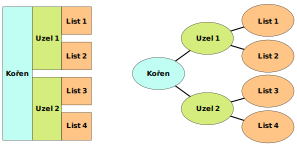
\includegraphics[width=140mm]{img/NUMATV/block-tree.pdf}
        \caption{Blokový strom (vlevo) a klasická grafová reprezentace stromu (vpravo)}
        \label{block-tree}
    \end{figure}
    \item \emph{Zkrácená topologie} - Reprezentace topologie s pouze nejdůležitějšími částmi pro topologickou vizualizaci od NUMA TV. Jedná se o třívrstvou strukturu, kde v první vrstvě jsou logické indexy NUMA uzlů, v druhé vstvě jsou logické indexy jader, ve třetí vrstvě jsou logické indexy procesorů spárovány s OS indexy procesorů.
    \item \emph{C} - Zkratka označující jádro v topologickém stromu, často zobrazováno se svým logickým indexem.
    \item \emph{Jádro} - Topologická struktura v Hwlocu obsahující jeden či více procesorů a která je obsažena v NUMA uzlech. Na systémech bez hyperthreadingu je tento termín zaměnitelný s procesorem.
    \item \emph{GL plocha} - kreslící OpenGL plocha používaná KernelSharkem na kreslení CPU grafů a grafů procesů.
    \item \emph{Logický index} - Index dán části topologie během jejího zkoumání Hwlocem. Společně s typem objektu (PU, jádro, NUMA uzel) pak tvoří unikátní identifikátor komponenty v dané topologii.
    \item \emph{NN} - Zkratka označující NUMA uzel v topologického stromu, často zobrazován se svým logickým indexem.
    \item \emph{NUMA TV} - Zkratka pro \uv{NUMA Topology Views}.
    \item \emph{NUMA TV kontext} - Konfigurační objekt modifikace, který se stará o konfiguraci NUMA TV pro každý otevřený stream, tj. cestu k souboru topologie, kterou má stream načtenou (pokud vůbec), a který typ pohledu chce stream použít při načtené topologii.
    \item \emph{OS index} - Index přidělen hardwarové komponentě operačním systémem. Nerespektuje topologii a pro vizualizace není moc užitečný. Tyto indexy používá KernelShark pro nápisy u CPU grafů, tj. pokud máme zobrazen graf pro CPU 0, tak \uv{0} je OS indexem daného procesoru.
    \item \emph{(Procesorový) modul} - Fyzické místo, kde jsou instalovány procesory (dle Hwlocu). Také součást topologie v Hwlocu, může obsahovat jeden i více NUMA uzlů, zároveň jeden modul může být součástí jednoho i více NUMA uzlů.
    \item \emph{PU/procesor} - Hwloc termín pro to samé, co jsou podle KernelSharku CPU. Mohou být seskupeny v jádru, každé jádro má aspoň jeden PU. PU je zkratka z anglického \uv{processing unit}.
    \item \emph{Topologie} - Struktura s detailní organizací paměťových modulů, procesorů, jiných zařízení na stroji/systému a obsahující nějaké dalších informace, jako například jméno stroje či celková paměť. Tuto strukturu dokáže zachytit Hwloc.
    \item \emph{Úlohová výplň} - Dodatečný prázdný prostor pod topologickým stromem v topologické ploše. Je přítomen pokud KernelShark ukazuje grafy úloh pro nějaký stream.
    \item \emph{Topologický strom} - Skupina Qt objektů, které dohromady tvoří blokový strom bez kořene, jehož první vrstvou jsou NUMA uzly, po nich je vrstva jader, které tvoří listy stromu. Topologické stromy jsou vždy součástí topologické plochy. Topologické stromy NUMA TV vždy vytváří z nějaké zkrácené topologie. Pokud zkrácená topologie nemá více než jeden NUMA uzel, pak se vrstva NUMA uzlů nezobrazuje.
    \item \emph{Vizualizace topologie} - V NUMA TV zaměnitelné s topologickým stromem.
    \item \emph{Topologická plocha} - Qt plocha s topologickým stromem a možnou úlohovou výplní. Je součástí wrapperu topologcké plochy. Lze přímo namapovat na třídu v kódu: \texttt{KsStreamTopoWidget}
    \item \emph{Pohled/typ pohledu} - výčtová třída pro vybrání způsobu zobrazení topologie v KernelSharku. NUMA TV definuje dva pohledy:
    \begin{itemize}
        \item Výchozí pohled, který ignoruje topologii. Pokud jso všechny pohledy nastaveny na výchozí, pak NUMA TV není v hlavním okně aktivní, tj. hlavní okno zobrazuje to samé, co bylo zobrazování před touto modifikací.
        \item \uv{NUMA tree}/stromový pohled, který pro topologii zobrazí topologický strom v topologické ploše.
    \end{itemize}  
    \item \emph{Wrapper topologické plochy} - Nalevo od GL plochy, obsahuje topologickou plochu. Existuje z implementačních důvodů.
\end{itemize}

%%%%%%%%%%%%%%%%%%%%%%%%%%%%%%%%%%%%%%%%%%%%%%%%%%%%%%%%%%%%%%%%%%%%%%%
\section{Analýza}
Tato sekce se pokusí zachytit postup, kterým se dostaneme k implementaci řešení. Jedná se o techničtější analýzu než analýza z kapitoly \emph{Obecná analýza a stanovení požadavků}. Zároveň se někdy odkážeme na Couplebreak a části jeho řešení, abychom se zbytečně neopakovali.

\subsection{Hwloc}
Chtěli bychom-li začít se zobrazováním dat topologie od Hwlocu, musíme si nejprve uvědomit, že se jedná o vylepšení, které přidá ke KernelSharku novou závislost, právě Hwloc. Toho jednoduše docílíme editací souborů sestavení pro CMake. Naštěstí pro nás dává dokumentace Hwlocu \cite{Hwloc-Docs} přímý návod, jak dodání závislosti docílit. Nám tedy stačí řídit se dokumentací a CMake instrukce překopírovat, zkontrolovat a drobně upravit pro KernelShark. Verzi Hwlocu vybereme co možná nejnvější, tj. verzi 2.11.

Na řadu přichází nahrání topologie z XML souboru do datové struktury, se kterou pak může Hwloc pracovat. Dokumentace nám opět pomůže a my můžeme přes Hwloc funkce a makra rovnou načíst XML soubor jako topologii. V té si nejprve získáme všechny OS indexy procesorů/PU a poté si přes každý z nich zjistíme i kterému jádru patří a kterému NUMA uzlu patří. Logické indexy PU, jader a NUMA uzlů si pak uložíme do zkrácené topologie. Abychom neztratili spojení mezi logickými indexy procesorů a jejich OS indexy, uložíme si do zkrácené topologie i OS indexy pro PU. Zkrácenou topologii můžeme implementovat pomocí neseřazených map a indexy můžeme reprezentovat pomocí celých čísel. Zkrácenou topologii použijeme proto, že Hwloc topologie obsahuje informace navíc, které nás u NUMA TV nezajímají, například uspoádání cache pamětí, nebo jméno stroje, na kterém byla topologie zachycena.

\subsection{Hlášení chyb}

Během nahrávání topologie se může stát nějaká chyba, například nebyl XML soubor ve správném formátu. I ve zbytku modifikace pak mohou nastat chvíle, kdy bude potřeba ošetřit a ohlásit nějakou chybovou či informační situaci. KernelShark sám výjimky nevyhazuje, namísto toho používá zprávy v terminálu nebo informační dialogy. NUMA TV bude používat návratové kódy a psaní do terminálu pro hlášení nějak zajímavých situací, jako třeba chyb.

\subsection{Konfigurační dialog}
\label{numatv-cfg-subsec}

Poté, co jsme schopni pracovat s Hwlocem a získat si pro nás zajímavá data, se můžeme začít soustředit vytvoření konfigurace NUMA TV. Začneme GUI pro uživatelskou interakci s konfigurací. Zde si můžeme i rozmyslet, co bude součástí konfigurace, kterou bude tento dialog měnit.

Všimněme si podobností s konfigurací pro Couplebreak \ref{cbreak-cfg-subsec}. I v této modifikaci chceme mít nastavení pro každý stream zvlášť. Můžeme se tedy konfiguračním dialogem Couplebreaku inspirovat a pozměnit jenom to, co pro každý ze streamů konfigurujeme. Naše cíle vyžadují alespoň konfigurovatelnou cestu k XML souboru topologie a typ pohledu, tj. \uv{jak naložit s načtenou topologií}.

Pohledy navíc cíle definují dva, výchozí a stromový. Výchozí pohled už z názvu napovídá, že bude výchozí hodnotou konfigurace pro pohledy. Pohledy můžeme implementovat přes rádiová tlačítka, pak budeme schopni mít vybranou jen jednu možnost pro nějakou skupinu tlačítek.

Výběr XML souboru lze zjednodušit použitím souborového dialogu od Qt a filtrovat pro soubory s příponou \texttt{.xml}. My pak jenom musíme vytvořit nějaké vybírací \texttt{Select} tlačítko, kterým souborový dialog vyvoláme. Ze souborového dialogu pak uložíme cestu k souboru XML jako textový řetězec. Ten pak uživateli zobrazíme, aby bylo jasné, že nějaká topologie byla vybrána. Na vymazání vybrané cesty pak dodáme tlačítko \texttt{Clear}. Výchozí hodnotou cesty k souboru bude přirozeně prázdný text. 

Speciální pozornost dáme tlačítku \texttt{Apply}. To totiž nejenže změny aplikuje, ale před aplikací i zkontroluje některé požadavky, které cíle požadují. Pokud je vybrán stromový pohled, ale nebyl vybrán topologický soubor, pak konfigurace vynutí pohled výchozí, jelikož není co zobrazovat ve stromovém pohledu. Pokud vybereme soubor s topologií o N CPU, ale stream, kterému toto konfigurujeme má M CPU a zároveň M se nerovná N, pak konfigurace opět použije výchozí pohled a uživatel bude o nevhodném souboru topologie informován na chybovém výstupu. Tlačítko \texttt{Cancel} může fungovat jako dřív, tedy prostě dialog zavře bez použití změn.

Tlačítko vyvolávající konfigurační dialog umístíme vedle tlačítka pro konfigurační okéno Couplebreaku, tj. do submenu \texttt{Tools}.

\subsection{Konfigurace NUMA TV}

V předchozí podsekci jsme si už trochu seznámili s tím, jak se bude konfigurace chovat, hlavně z grafického pohledu. Nyní se zamyslíme nad tím, jak by se měla chovat mimo grafické prostředí.

Nejprve se zamyslíme nad tím, jak reprezentovat pohledy. My implementujeme jenom stromový pohled na NUMA topologii, ale teoreticky jich může být více, například pohled na procesorové moduly. Proto pohledy implementujeme jako výčtový typ. Tak se omezíme jen na nějakou konečnou množinu hodnot a budeme mít kódu zřetelněji popsané speciální číselné hodnoty.

Dokud uživatel nezmění konfiguraci v dialogu z výchozích hodnot, pak NUMA TV nebude ukládat žádnou konfiguraci pro stream, jelikož by to bylo zbytečné. Pokud ale uživatel vybere validní XML soubor s topologií, pak se situace mění. Aplikace konfigurace pak donutí NUMA TV vytvořit novou konfiguraci pro stream, včetně interpretace topologického XML sobuoru Hwlocem. Po ní nám zbyde zkrácená topologie, kterou také uložíme do konfigurace pro stream. Z toho nám vyplývá, že datová struktura konfigurace NUMA TV pro nějaký stream bude obsahovat prvky pro uložení cesty k XML souboru, uložení typu pohledu a uložení zkrácené topologie.

Pokud uživatel vymaže v konfiguračním dialogu cestu k topologickému souboru, pak není konfigurace pro stream potřeba. Pro nás to znamená návrat k výchozím hodnotám konfigurace (i kdyby byl vybrán stromový pohled, tak bez cesty k souboru topologie toto NUMA TV změní na výchozí pohled). Abychom zbytečně neukládali nepotřebnou konfiguraci, tak ji v této situaci smažeme.

Dalším problémem, co vyřešíme, je aktualizace topologie. Ta se stane, když uživatel změní cestu k topologickému souboru a nebo změní typ pohledu v konfiguračním dialogu a změny aplikuje. Pokud změní cestu, pak lze považovat starou konfiguraci topologie za zbytečnou a tak ji smažeme. Můžeme ji pak kompletně nahradit novou konfigurací. Pokud se změnil jen pohled, pak změníme jen ten. V každém případě ale požádáme  NUMA TV o překreslení topologických vizualizací (vizualizační část je popsána v nižší sekci \ref{numatv-grt}). Pokud je topologie nějak nevalidní (případy popsány v sekci o konfiguračním dialogu výše \ref{numatv-cfg-subsec}), pak návratovým kódem rozhodneme, jak se má KernelShark zachovat tj. jestli má do terminálu napsat nějakou chybovou zprávu.

Nakonec, namísto ukládání konfigurací ke každému streamu zvlášť si pořídíme manažera konfigurací, tzv. NUMA TV (konfigurační) kontext. Ten si bude pro každý stream pamatovat jeho specifickou konfiguraci. Krom toho bude mít i API pro přidávání, odebírání, a aktualizaci konfigurací pro každý stream. Jelikož mezi streamy mohou být \uv{díry}, tj. ne každý stream musí mít aktivní NUMA TV konfiguraci, bude nejlepší i toto vyřešit mapou, klidně i nesetříděnou.

\subsection{Grafická reprezentace topologie/GRT}
\label{numatv-grt}
[TODO: tohle] %%% Turing-head |vvv|
Topostrom (barvy a interaktivita, vzhled topostromu celkově)...

CPU grafy a grafy úloh...

cpuReDraw + taskReDraw...

Reorganizace grafů dle topologie...

Místo pro GRT (+ velikost + nemožnost scrollovat + updateGeom)...

Spolupráce s filtry...

Schovávání topologie...

\subsection{Životnosti}
Vše patří KsTraceGraph...

Vše umírá v napsaných konstruktorech správně...

\subsection{Relace}
Relace implementujeme mnohem snadněji než u Couplebreaku. NUMA TV uloží pod identifikátor streamu vybraný typ pohledu a cestu k XML souboru (nebo žádnou cestu neuloží v případě nevybraného souboru v konfiguraci). Inspirovat se můžeme ostatním kódem pro ukládání relace, například pro ukládání Markerů A a B. A stejně se inspirujeme i pro načítání NUMA TV z relačního souboru.

Nyní zbývá vybrat momenty, kdy ukládat NUMA TV a hlavně kdy relační data pro modifikaci načítat. Nelze načítat kdykoliv, jelikož bychom jinak nezastihli vykreslení CPU grafů, tedy i jejich možnou reorganizaci, což by vizualizaci úplně pokazilo. Načítat relační data proto budeme před načtením grafu, abychom vykreslení CPU stihli. Ukládání není závislé na pořadí ukládání ostatních částí relace, ale kvůli symetrii s načítáním jej zařadíme před ukládání grafů.

%----------------------------------------------------------------------

\subsection{Zamítnutá alternativní řešení}
Tato část je souhrnem několika nápadů, které se objevily během vymýšlení řešení či během implementace, ale byly nakonec zavrženy z různých důvodů. Představen bude jak návrh řešení, tak důvod zamítnutí.

\subsubsection*{Konfigurační kontext jako singleton}
Až moc dlouho jako prototyp, velmi nebezpečný vzor...

\subsubsection*{Kreslení stromu do OpenGL plochy}
Příšerné, nikdy to tak nedělejme...

\subsubsection*{Graf vytvořen přes QTreeWidget}
Nedostatečné schopnosti a layout nebyl vhodný, reimplementace by byla šílená

\subsubsection*{Zobrazení procesorů a stroje v topologickém stromě}
Zbytečné, ačkoliv stream to aspoň ukotvoval jako strom - nicméně více místa = více radosti...

\subsubsection*{Vlastní zpracování XML souboru}
Pro humor, tohle by byla prostě šílenost...

\subsubsection*{Topologie jako součást datové struktury streamu}
Zbytečné omezení na jazyk C...

\subsubsection*{Topologické zobrazení přítomno neustále}
Zbytečné plýtvání místem...

\subsubsection*{Skládání částí stromu}
Zbytečně komplikované, zbytečná fnkcionalita, která se jen plete pod nohy existujícímu řešení přes menu, ale měla i svá plus...

%%%%%%%%%%%%%%%%%%%%%%%%%%%%%%%%%%%%%%%%%%%%%%%%%%%%%%%%%%%%%%%%%%%%%%%
\section{Vývojová dokumentace}
Cíle/úvod této sekce...

\subsection{Modifikované a nové soubory}
Modifikace používá značku \texttt{NUMA TV} v ohraničujících komentářích pro změny. Níže je abecedně seřazený seznam souborů spojených s modifikací spolu s krátkým popiskem změn či novinek uvnitř souboru.
\begin{itemize}
    \item \emph{(src/)CMakeLists.txt} -
    \item \emph{KsMainWindow.cpp/hpp} - 
    \item \emph{KsNUMATopologyViews.cpp/hpp} -
    \item \emph{KsPlotTools.cpp/hpp} - 
    \item \emph{KsSession.cpp/hpp} -
    \item \emph{KsTraceGraph.cpp/hpp} - 
    \item \emph{KsWidgetsLib.cpp/hpp} -
\end{itemize}

\subsection{Struktura modifikace}
Velké dělení na \emph{Konfiguraci} a \emph{Vizualizaci}. Vše vlastí objekt KsTraceGraph, kromě konfiguračního dialogu, který je vázán jenom na hlavní okno KernelSharku hierarchií oken.

Dělení Konfigurace:
\begin{itemize}
    \item \emph{Konfigurační kontext} -
    \item \emph{Konfigurační dialog} -
    \item \emph{Vytváření zkrácených topologií z Hwlocu} -
    \item \emph{Dotazy na topologii} -
    \item \emph{Relace} -
\end{itemize}

Dělení Vizualizace (modul je i jeden grafický prvek):
\begin{itemize}
    \item \emph{Topologický strom} -
    \item \emph{Prostor pro topologický strom} -
    \item \emph{Skrývající tlačítko} -
    \item \emph{Přerovnání CPU} -
\end{itemize}

%%%%%%%%%%%%%%%%%%%%%%%%%%%%%%%%%%%%%%%%%%%%%%%%%%%%%%%%%%%%%%%%%%%%%%%
\section{Uživatelská dokumentace}

\begin{code}

\subsection{Konfigurace}

To access NUMA TV's confguration, navigate to `Tools > NUMA Topology Views`
button in the toolbar. If no stream was loaded, an error pop-up will be shown
and nothing will happen otherwise.

With a loaded stream, the NUMA TV configuration dialog will be shown,
with a brief explanation of what to do in this window and in the lower half will be
a list of opened streams' NUMA TV configurations, namely what topology file to
load data from and what type of topology view should be used for this stream.
There are also two buttons, "Clear" and "Select...". Clear clears current
configuration's selected topology file (just the filepath to it, not the file
itself). Select button will open up a file dialog, which either starts in the user's
Documents directory or in the directory of the currently applied topology file
(applied = program already loaded this topology file and uses it for a stream).

At the very bottom are two buttons, "Apply" and "Close". Close will ignore any
changes to the configuration done in the window and close the dialog. Apply will
attempt to either create or update chosen stream's topology configuration with
the chosen values.

Beware that if the chosen topology in a file has a different amount of PUs than
KernelShark detected CPUs in its trace file, creation or update of this topology
configuration is ignored (old values remain or the default choice of no topology
file and DEFAULT view). Topology configuration changes will also be ignored if
no actual topology file was chosen (cleared the path or it has been deleted in
between choosing it and applying the changes), yet the NUMA tree view was set.

Applying an empty filepath current configuration of a stream and program will
default to using DEFAULT view with no topology file.

Currently, only NUMA topology tree view is supported, along with the DEFAULT view,
which does what KernelShark always has.

Reopening the configuration dialog will show applied configuration values
(currently in use by the program).

See figure 2 for a session where no topologies are loaded and figure 3 for
a session where one topology is loaded.

![Figure 2](./images/numatv-2.png)
Figure 2.

![Figure 3](./images/numatv-3.png).
Figure 3.

\subsection{GUI}

\subsubsection{Kde najít NUMA TV}

NUMA Topology Views are at first glance not present in the program. This is by
design, as the modification is supposed to be hidden until needed. To see the
modification in action, first open a stream. Then, open and use the configuration
dialog as outlined above.

The wrapper topology widget will be shown if at least one stream requested a
non-DEFAULT topology view. If any CPUs are shown on the GL widget, there will
also be a topology tree present for the streams that requested a NUMA tree view.
Streams configured to use the DEFAULT view only have blank spaces in as their
topology widget. 

\subsubsection{Topologický strom}
The topology tree is a block tree, which is vertically starts at the top of the
start of CPU graphs in the GL widget and vertically ends at the last of those
graphs. If there are only tasks being drawn, there will be blank white space
instead. The topology tree will include only nodes relevant to the CPUs shown in
the GL widget (so if out of 8 CPUs, only 3 are marked as to show their graphs,
then the topology tree will be constructed with cores and NUMA nodes of those
three CPUs). If the topology has only single NUMA node detected (in which case
there is no actual NUMA topology present), the node will be hidden (only Cores
will be visible).

If more streams are opened, each tree starts at its respective stream's CPU
graphs.

Core nodes of the tree will be colored the average color of its CPUs (these colors
are defined by KernelShark), NUMA nodes are colored from averages of core node
colors. If a color is deemed too dark, white text is used for their labels,
otherwise the nodes use black text color.

\subsubsection{Synchronizace rolování s plochou grafu}

While the wrapper topology widget sits in a scrollable area, to retain consistency with
KernelShark's method of scrolling vertically through a graph, no mouse wheel events
are processed by it. Instead, the scrolling area moves the same amount as GL widget's
scrolling area, when its vertical scrollbar's value changes.

If KernelShark's main window is too narrow, a horizontal scroll bar also appears, but
at that point, it is recommended to resize the main window of the program.

\subsubsection{Přeuspořádání CPU grafů}

If a topology determined that CPUs adhere to a different ordering than OS indices indicate,
NUMA TV will rearrange the CPU graphs in the GL widget to properly connect to the topology tree
of a stream. In DEFAULT view, KernelShark orders CPUs by their OS indices, with a NUMATREE view,
they are ordered by their NUMA node's logical index, then their core's logical index and lastly
by their logical index (i.e. a sorted sequence could look like (0, 0, 20), (0, 0, 60), (0, 1, 1),
(1, 5, 2), (1, 5, 3), where first number in the vector is NUMA node's logical index, followed
by the core's logical index, ending with a PUs logical index).

KernelShark graph will still label CPUs with their OS indices.

Rearrangements may happen only if a non-DEFAULT view is chosen for a stream and rearrange CPU
graphs only of that stream. A rearrangament may happen any time the CPU graphs are redrawn.

See figure 4 for a stream with CPU graphs ordered by OS indices, then compare with figure 5's
reordered CPU graphs.

![Figure 4](./images/numatv-4.png)
Figure 4.

![Figure 5](./images/numatv-5.png)
Figure 5.

\subsubsection{Skrývající tlačítko}

Hide button is a green button on the left of the wrapper topology widget. Clicking on it
hides the wrapper topology widget along with all topology trees (figure 6). Clicking on
it again makes the wrapper topology widget and its trees visible again (figure 7).
Accompanied with hidden/shown states are characters on the button: ">" for hidden
and "<" for shown.

This button is shown only if there's at least one stream requesting a non-DEFAULT topology view.
Upon any load of topology requesting a non-DEFAULT view, the wrapper topology widget is not
hidden (figure 7).


![Figure 6](./images/numatv-6.png)
Figure 6.

![Figure 7](./images/numatv-7.png)
Figure 7.

\subsubsection{Plovoucí popisky uzlů stromu}

Hovering with the mouse cursor over a topology tree node and letting it stay there for a little while
shows a tooltip with the current node's full name, e.g. hovering over a node labeled 'NN 1' will show
"NUMA Node 1" (figure 8).

Purpose of this is to allow short labels for the nodes, while preserving a quick way for the user to
understand what a certain node is.

![Figure 8](./images/numatv-8.png)
Figure 8.

\subsection{Popora relací}

NUMA Topology Views configuration can be saved in a session using new API of KsSession. Each stream has their view and
topology file path saved.

Importing a session automatically draws topology widgets, if any are desired.

\subsection{Nová API}

NUMA TV presents among new classes also four new global functions:
- `numatv_count_PUs`: This function counts the number of PUs in a brief topology.
- `numatv_count_cores`: This function counts the number of cores in a brief topology.
- `numatv_filter_by_PUs`: This functions returns a brief topology, where its members contain or
  are PUs given in a vector. This function is very useful when some CPU graphs are hidden - by
  filtering the brief topology, we get a brief topology where only the visible CPUs are present,
  same for their cores and NUMA nodes.
- `numatv_stream_wants_topology_widget`: This function checks whether a stream is requesting a
  non-DEFAULT view in its configuration in the given NUMA TV context

Any other API that got introduced is either explicitly labeled with "numatv" ot "topology" or "topo"
somewhere (letters can be uppercase). If not, it belongs to a type with that label or a header
file with that label.

Use carefully.

\subsection{Bugy a chyby}

Qt may sometimes complain about recursive call when clicking the Load button in the configuration dialog. This has no bearing
on actual work of the program, as Qt makes sure to detect these calls and stop them. This may happen if the Load button
is clicked too fast.

No others are known to the author. But the modification was rather significant and there are always possibilites something
went wrong in secret.
\end{code}

%%%%%%%%%%%%%%%%%%%%%%%%%%%%%%%%%%%%%%%%%%%%%%%%%%%%%%%%%%%%%%%%%%%%%%%
\section{Rozšíření}
Cíle/úvod této sekce...

\subsubsection*{Více pohledů}
Package view, něco spešl, ALE nutno vyřešit \ref{nerozšiřitelnost}...

\subsubsection*{Konfigurační dialogy by mohly být zobecněny}
Couplebreak a NUMA TV mají v podstatě stejnou šablonu, bylo by lepší ji zobecnit...

%%%%%%%%%%%%%%%%%%%%%%%%%%%%%%%%%%%%%%%%%%%%%%%%%%%%%%%%%%%%%%%%%%%%%%%
\section{Kritika}
V této sekci autor kriticky zhodnotí své řešení. Každá kritika má nadpis a popis a dále buď obsahuje obranu proti ní, nebo souhlas s předneseným problémem.

\subsubsection*{Nerozšiřitelnost}
\label{nerozšiřitelnost}
Primárně pro NUMA topologii, nedostatečný vhled dopředu pro další viewtypes, ať už v GUI nebo v konfiguraci...

\subsubsection*{Nevhodné umístění třídy \texttt{KsStreamNUMATopology}}
Mělo to mít vlastní soubor nebo do NUMATV souboru...

\subsubsection*{Kostrbaté vložení závislosti do \texttt{CMakeLists.txt} KernelSharku}
Ale je to oficiální...

\subsubsection*{Nemožnost upravovat aktivní topologie}
Místo toho create + delete only...

\subsubsection*{Výjimky místo návratových kódů}
KernelShark to tak nedělá...

\subsubsection*{Porušení SRP}
Zas tak moc ne, furt to zlepšuje analýzu, nicméně chápu, odkud míříme...

\subsubsection*{Orientace a velikost popisků topologického stromu}
Mohlo by být větší/tučné/vertikální/rotované...

\subsubsection*{Barva uzlů topologického stromu}
Avg z toho většinou udělá šedou/hnědou... mohlo by být jinak...

\subsubsection*{Konfigurace a widget v oddělených mapách}
Nemuselo by být, ale dává smysl...

\subsubsection*{Malá interaktivita topologického zobrazení}
A to vůbec nevadí...ale samozřejmě by šlo něco takového dodat...

\subsubsection*{Používání C ukazatelů}
Pravda, nejsou moc bezpečné, ale KernelShark to často dělá a Qt si s nimi umí poradit...

\subsubsection*{Dialogy namísto standardních výstupů}
Grafická aplikace, ne nutně bude vždy uživatel mít přístup k jejímu terminálovému výstupu...

%%%%%%%%%%%%%%%%%%%%%%%%%%%%%%%%%%%%%%%%%%%%%%%%%%%%%%%%%%%%%%%%%%%%%%%
\section{Zhodnocení splnění požadavků}
Obecné požadavky hlavně + možná nějaká porušení + splnění vlastních cílů...